\documentclass{article}
\nocite{*}


%--PASTE INTO MAIN FILE--
% \documentclass{article}
% %--PASTE INTO MAIN FILE--
% \documentclass{article}
% %--PASTE INTO MAIN FILE--
% \documentclass{article}
% \input{TexBase/DocumentBase.tex}
% \end{document}


\usepackage[margin = 0.7in]{geometry}
\usepackage{graphicx}
\usepackage{graphics}
\usepackage[T1]{fontenc}
\usepackage[polish]{babel}
\usepackage[utf8]{inputenc}
\usepackage{float}
\usepackage{tabularx}
\usepackage[table,xcdraw]{xcolor}
\usepackage{lipsum}
\usepackage{titlesec}
\usepackage{minted}
\usepackage{xcolor}
\usepackage{caption}
\usepackage{enumitem}
\usepackage{csvsimple}
% \usepackage{natbib}
\usepackage{blindtext}
\usepackage{numprint} % rounding
\usepackage[round-precision=3,round-mode=figures, scientific-notation=true]{siunitx} %scientific notation
\usepackage[hidelinks]{hyperref}
\usepackage{url}
\usepackage{bm} %bold for math
\usepackage[]{booktabs}
\usepackage{tabularray}
\usepackage{multirow}

%\title{}
\author{Michał Dziedziak}
\date{\today}


\titlespacing\section{0pt}{12pt plus 4pt minus 2pt}{0pt plus 2pt minus 2pt}
\titlespacing\subsection{0pt}{12pt plus 4pt minus 2pt}{0pt plus 2pt minus 2pt}
\titlespacing\subsubsection{0pt}{12pt plus 4pt minus 2pt}{0pt plus 2pt minus 2pt}
\setlength{\parskip}{\baselineskip}%
\setlength{\parindent}{0pt}%

\newcommand{\squeezeup}{\vspace{-5mm}}


\begin{document}

\begin{titlepage}
    \begin{center}
        \vspace*{5cm}
        \rule{500pt}{1pt}\\
        \vspace*{0.5cm}
        \LARGE
        \textbf{Kolor na budowie}\\
        \Large
        \vspace*{0.5cm}
        \rule{500pt}{1pt}
    \end{center}

    \vspace*{10cm}

    {\raggedright
        \large
        \textbf{Autor sprawozdania:} Michał Dziedziak 263901\\
        \textbf{Imię i Nazwisko prowadzącego kurs:} dr inż. Agata Migalska\\
        \textbf{Dzień i godzina zajęć:} Środa P, 17:05 - 18:45
    }
\end{titlepage}


\tableofcontents
\listoftables
\listoffigures


\newpage


% \begin{table}[H]
%     \centering
%     \begin{tabular}{|c|c|c|c|}%
%         \hline
%         \bfseries Numer iteracji & \bfseries Czas zalezienia rozwiązania [ms] & Koszt ścieżki & Błąd względny% specify table head
%         \csvreader[head to column names]{Csv/BestPathTest_SimulatedAnnealing_LINEAR_ftv47.csv}{}% use head of csv as column names
%         {\\\hline\Iteration & \num{\TimeInMiliSeconds} & \Cost & \num[round-precision=2, round-mode=places, scientific-notation=false]{\Error}\%}% specify your columns here
%         \\\hline    
%     \end{tabular}
%     \caption{}
%     \label{tab:}
% \end{table}

% \begin{figure}[H]
%     \centering
%     \resizebox{\columnwidth}{!}{%
%     \includegraphics{}%
%     }
%     \caption{}
%     \label{fig:}
% \end{figure}


% \bibliographystyle{plainnat}
% \bibliography{Bibliography}
% \end{document}


\usepackage[margin = 0.7in]{geometry}
\usepackage{graphicx}
\usepackage{graphics}
\usepackage[T1]{fontenc}
\usepackage[polish]{babel}
\usepackage[utf8]{inputenc}
\usepackage{float}
\usepackage{tabularx}
\usepackage[table,xcdraw]{xcolor}
\usepackage{lipsum}
\usepackage{titlesec}
\usepackage{minted}
\usepackage{xcolor}
\usepackage{caption}
\usepackage{enumitem}
\usepackage{csvsimple}
% \usepackage{natbib}
\usepackage{blindtext}
\usepackage{numprint} % rounding
\usepackage[round-precision=3,round-mode=figures, scientific-notation=true]{siunitx} %scientific notation
\usepackage[hidelinks]{hyperref}
\usepackage{url}
\usepackage{bm} %bold for math
\usepackage[]{booktabs}
\usepackage{tabularray}
\usepackage{multirow}

%\title{}
\author{Michał Dziedziak}
\date{\today}


\titlespacing\section{0pt}{12pt plus 4pt minus 2pt}{0pt plus 2pt minus 2pt}
\titlespacing\subsection{0pt}{12pt plus 4pt minus 2pt}{0pt plus 2pt minus 2pt}
\titlespacing\subsubsection{0pt}{12pt plus 4pt minus 2pt}{0pt plus 2pt minus 2pt}
\setlength{\parskip}{\baselineskip}%
\setlength{\parindent}{0pt}%

\newcommand{\squeezeup}{\vspace{-5mm}}


\begin{document}

\begin{titlepage}
    \begin{center}
        \vspace*{5cm}
        \rule{500pt}{1pt}\\
        \vspace*{0.5cm}
        \LARGE
        \textbf{Kolor na budowie}\\
        \Large
        \vspace*{0.5cm}
        \rule{500pt}{1pt}
    \end{center}

    \vspace*{10cm}

    {\raggedright
        \large
        \textbf{Autor sprawozdania:} Michał Dziedziak 263901\\
        \textbf{Imię i Nazwisko prowadzącego kurs:} dr inż. Agata Migalska\\
        \textbf{Dzień i godzina zajęć:} Środa P, 17:05 - 18:45
    }
\end{titlepage}


\tableofcontents
\listoftables
\listoffigures


\newpage


% \begin{table}[H]
%     \centering
%     \begin{tabular}{|c|c|c|c|}%
%         \hline
%         \bfseries Numer iteracji & \bfseries Czas zalezienia rozwiązania [ms] & Koszt ścieżki & Błąd względny% specify table head
%         \csvreader[head to column names]{Csv/BestPathTest_SimulatedAnnealing_LINEAR_ftv47.csv}{}% use head of csv as column names
%         {\\\hline\Iteration & \num{\TimeInMiliSeconds} & \Cost & \num[round-precision=2, round-mode=places, scientific-notation=false]{\Error}\%}% specify your columns here
%         \\\hline    
%     \end{tabular}
%     \caption{}
%     \label{tab:}
% \end{table}

% \begin{figure}[H]
%     \centering
%     \resizebox{\columnwidth}{!}{%
%     \includegraphics{}%
%     }
%     \caption{}
%     \label{fig:}
% \end{figure}


% \bibliographystyle{plainnat}
% \bibliography{Bibliography}
% \end{document}


\usepackage[margin = 0.7in]{geometry}
\usepackage{graphicx}
\usepackage{graphics}
\usepackage[T1]{fontenc}
\usepackage[polish]{babel}
\usepackage[utf8]{inputenc}
\usepackage{float}
\usepackage{tabularx}
\usepackage[table,xcdraw]{xcolor}
\usepackage{lipsum}
\usepackage{titlesec}
\usepackage{minted}
\usepackage{xcolor}
\usepackage{caption}
\usepackage{enumitem}
\usepackage{csvsimple}
% \usepackage{natbib}
\usepackage{blindtext}
\usepackage{numprint} % rounding
\usepackage[round-precision=3,round-mode=figures, scientific-notation=true]{siunitx} %scientific notation
\usepackage[hidelinks]{hyperref}
\usepackage{url}
\usepackage{bm} %bold for math
\usepackage[]{booktabs}
\usepackage{tabularray}
\usepackage{multirow}

%\title{}
\author{Michał Dziedziak}
\date{\today}


\titlespacing\section{0pt}{12pt plus 4pt minus 2pt}{0pt plus 2pt minus 2pt}
\titlespacing\subsection{0pt}{12pt plus 4pt minus 2pt}{0pt plus 2pt minus 2pt}
\titlespacing\subsubsection{0pt}{12pt plus 4pt minus 2pt}{0pt plus 2pt minus 2pt}
\setlength{\parskip}{\baselineskip}%
\setlength{\parindent}{0pt}%

\newcommand{\squeezeup}{\vspace{-5mm}}


\begin{document}

\begin{titlepage}
    \begin{center}
        \vspace*{5cm}
        \rule{500pt}{1pt}\\
        \vspace*{0.5cm}
        \LARGE
        \textbf{Kolor na budowie}\\
        \Large
        \vspace*{0.5cm}
        \rule{500pt}{1pt}
    \end{center}

    \vspace*{10cm}

    {\raggedright
        \large
        \textbf{Autor sprawozdania:} Michał Dziedziak 263901\\
        \textbf{Imię i Nazwisko prowadzącego kurs:} dr inż. Agata Migalska\\
        \textbf{Dzień i godzina zajęć:} Środa P, 17:05 - 18:45
    }
\end{titlepage}


\tableofcontents
\listoftables
\listoffigures


\newpage


% \begin{table}[H]
%     \centering
%     \begin{tabular}{|c|c|c|c|}%
%         \hline
%         \bfseries Numer iteracji & \bfseries Czas zalezienia rozwiązania [ms] & Koszt ścieżki & Błąd względny% specify table head
%         \csvreader[head to column names]{Csv/BestPathTest_SimulatedAnnealing_LINEAR_ftv47.csv}{}% use head of csv as column names
%         {\\\hline\Iteration & \num{\TimeInMiliSeconds} & \Cost & \num[round-precision=2, round-mode=places, scientific-notation=false]{\Error}\%}% specify your columns here
%         \\\hline    
%     \end{tabular}
%     \caption{}
%     \label{tab:}
% \end{table}

% \begin{figure}[H]
%     \centering
%     \resizebox{\columnwidth}{!}{%
%     \includegraphics{}%
%     }
%     \caption{}
%     \label{fig:}
% \end{figure}


% \bibliographystyle{plainnat}
% \bibliography{Bibliography}


\section{Wprowadzenie} %TODO
\section{Uczestnicy badania}
    \subsection{Analiza deskryptywna zmiennych demograficznych}
        \subsubsection*{Wiek}
        \begin{table}[H]
            \centering
            \caption{Opis deskryptywny wieku uczestników badania.}
            \begin{tabular}{|c|c|c|c|}%
                \hline
                \bfseries Miara & \bfseries Gogle przezroczyste & \bfseries Gogle czerwone & \bfseries Gogle żółte% specify table head
                \csvreader[head to column names]{./../res_tables/summaryAge.csv}{}% use head of csv as column names
                {\\\hline\Miara & \num{\T} & \num{\R} & \num{\Y}}% specify your columns here
                \\\hline    
            \end{tabular}
            \label{tab:summaryAge}
        \end{table}

        \begin{figure}[H]
            \centering
            \caption{Histogram dla wieku uczestników badania.}
            \resizebox{0.7 \columnwidth}{!}{%
            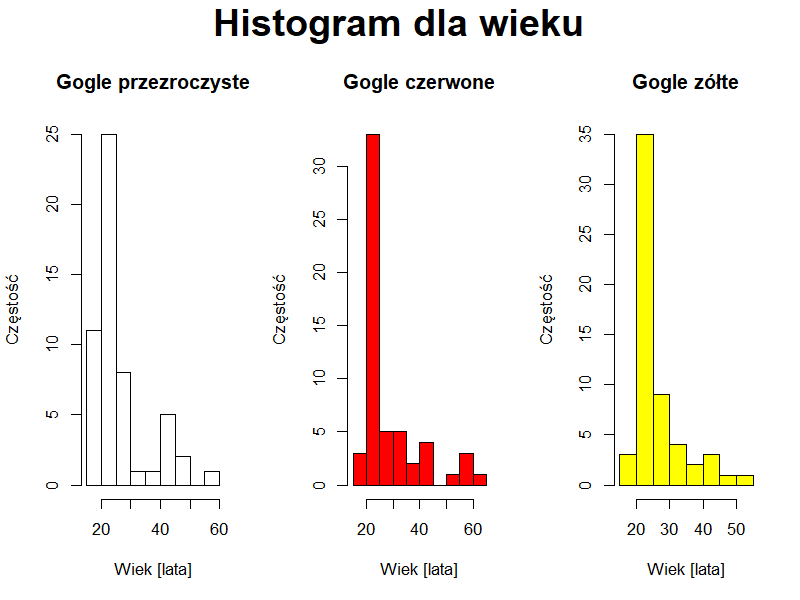
\includegraphics{./../res_plots/Histogram_dla_wieku.png}%
            }
            \label{fig:histAge}
        \end{figure}

        \begin{figure}[H]
            \centering
            \caption{Wykres pudełkowy dla wieku uczestników badania.}
            \resizebox{0.7 \columnwidth}{!}{%
            \includegraphics{./../res_plots/Wykres_pudełkowy_dla_wieku.png}%
            }
            \label{fig:boxAge}
        \end{figure}

        \subsubsection*{Doświadczenie zawodowe}
        \begin{table}[H]
            \centering
            \caption{Opis deskryptywny doświadczenia zawodowego uczestników badania.}
            \begin{tabular}{|c|c|c|c|}%
                \hline
                \bfseries Miara & \bfseries Gogle przezroczyste & \bfseries Gogle czerwone & \bfseries Gogle żółte% specify table head
                \csvreader[head to column names]{./../res_tables/summaryExperience.csv}{}% use head of csv as column names
                {\\\hline\Miara & \num{\T} & \num{\R} & \num{\Y}}% specify your columns here
                \\\hline    
            \end{tabular}
            \label{tab:summaryExperience}
        \end{table}

        \begin{figure}[H]
            \centering
            \caption{Histogram dla doświadczenia zawodowego uczestników badania.}
            \resizebox{0.7 \columnwidth}{!}{%
            \includegraphics{./../res_plots/Histogram_dla_doświadczenia_zawodowego.png}%
            }
            \label{fig:histExperience}
        \end{figure}


        \subsubsection*{Wyniki testu \textit{''health and safety''} (H\&S)}
        \begin{table}[H]
            \centering
            \caption{Opis deskryptywny wyników testu \textit{''health and safety''} (H\&S) uczestników badania.}
            \begin{tabular}{|c|c|c|c|}%
                \hline
                \bfseries Miara & \bfseries Gogle przezroczyste & \bfseries Gogle czerwone & \bfseries Gogle żółte% specify table head
                \csvreader[head to column names]{./../res_tables/summaryHSTestResults.csv}{}% use head of csv as column names
                {\\\hline\Miara & \num{\T} & \num{\R} & \num{\Y}}% specify your columns here
                \\\hline    
            \end{tabular}
            \label{tab:summaryHSTestResults}
        \end{table}

        \begin{figure}[H]
            \centering
            \caption{Histogram dla wyników testu \textit{''health and safety''} (H\&S) uczestników badania.}
            \resizebox{0.7 \columnwidth}{!}{%
            \includegraphics{./../res_plots/Histogram_dla_wyników_testu_H&S.png}%
            }
            \label{fig:histHSTestResults}
        \end{figure}

        \begin{figure}[H]
            \centering
            \caption{Wykres pudełkowy dla wyników testu \textit{''health and safety''} (H\&S) uczestników badania.}
            \resizebox{0.7 \columnwidth}{!}{%
            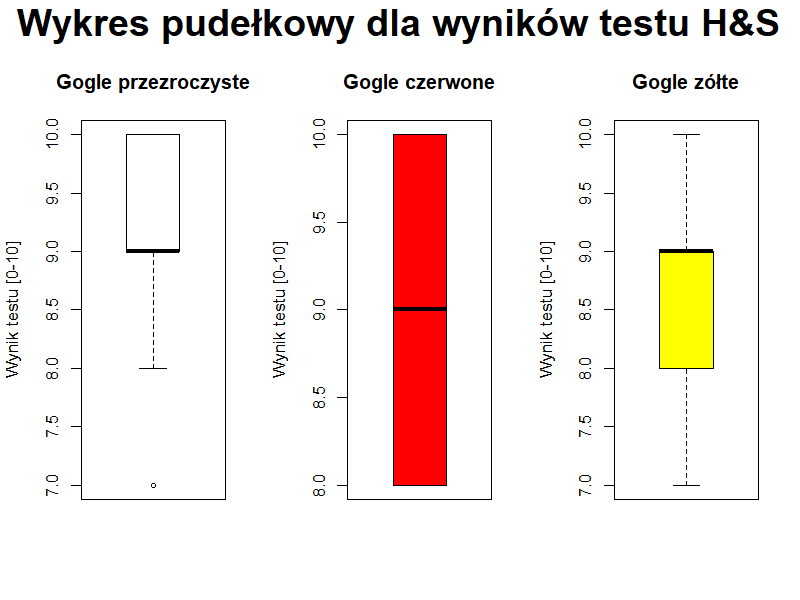
\includegraphics{./../res_plots/Wykres_pudełkowy_dla_wyników_testu_H&S.png}%
            }
            \label{fig:boxHSTestResults}
        \end{figure}

        \subsubsection*{Płeć}
        \begin{table}[H]
            \centering
            \caption{Opis deskryptywny płci uczestników badania.}
            \begin{tabular}{|c|c|c|c|}%
                \hline
                \bfseries Miara & \bfseries Gogle przezroczyste & \bfseries Gogle czerwone & \bfseries Gogle żółte% specify table head
                \csvreader[head to column names]{./../res_tables/summarySex.csv}{}% use head of csv as column names
                {\\\hline\Miara & \num{\T} & \num{\R} & \num{\Y}}% specify your columns here
                \\\hline    
            \end{tabular}
            \label{tab:summarySex}
        \end{table}

        \begin{figure}[H]
            \centering
            \caption{Histogram dla płci uczestników badania.}
            \resizebox{0.7 \columnwidth}{!}{%
            \includegraphics{./../res_plots/Histogram_dla_płci_(F=1,_M=2,_O=3).png}%
            }
            \label{fig:histEsx}
        \end{figure}


    \subsection{Czas noszenia gogli}
    \begin{table}[H]
        \centering
        \caption{Opis deskryptywny czasu noszenia gogli uczestników badania.}
        \begin{tabular}{|c|c|c|c|}%
            \hline
            \bfseries Miara & \bfseries Gogle przezroczyste & \bfseries Gogle czerwone & \bfseries Gogle żółte% specify table head
            \csvreader[head to column names]{./../res_tables/summaryTime.csv}{}% use head of csv as column names
            {\\\hline\Miara & \num{\T} & \num{\R} & \num{\Y}}% specify your columns here
            \\\hline    
        \end{tabular}
        \label{tab:summaryTime}
    \end{table}

    \begin{figure}[H]
        \centering
        \caption{Histogram dla czasu noszenia gogli uczestników badania.}
        \resizebox{0.7 \columnwidth}{!}{%
        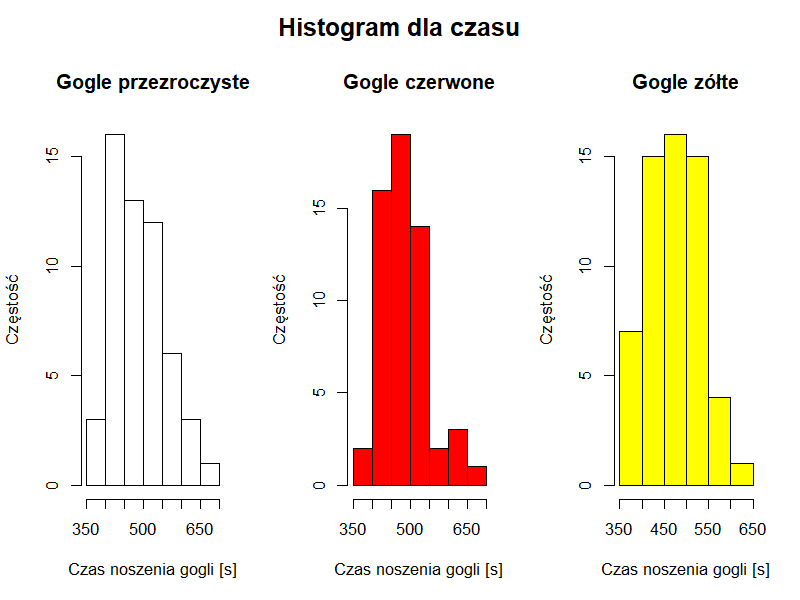
\includegraphics{./../res_plots/Histogram_dla_czasu.png}%
        }
        \label{fig:histTime}
    \end{figure}

    \begin{figure}[H]
        \centering
        \caption{Wykres pudełkowy dla czasu noszenia gogli uczestników badania.}
        \resizebox{0.7 \columnwidth}{!}{%
        \includegraphics{./../res_plots/Wykres_pudełkowy_dla_czasu.png}%
        }
        \label{fig:boxTime}
    \end{figure}

\section{Analiza TFD dla obiektu żółta torba (yellow bag)} %TODO
    \subsection{Hipotezy} %TODO
    \subsection{Analiza deskryptywna zmiennej}
    \begin{table}[H]
        \centering
        \caption{Opis deskryptywny zmiennej TFD dla obiektu żółta torba (yellow bag).}
        \begin{tabular}{|c|c|c|c|}%
            \hline
            \bfseries Miara & \bfseries Gogle przezroczyste & \bfseries Gogle czerwone & \bfseries Gogle żółte% specify table head
            \csvreader[head to column names]{./../res_tables/summaryTFD_yBag.csv}{}% use head of csv as column names
            {\\\hline\Miara & \num{\T} & \num{\R} & \num{\Y}}% specify your columns here
            \\\hline    
        \end{tabular}
        \label{tab:summaryTFD_yBag}
    \end{table}
    % \begin{figure}[H]
    %     \centering
    %     \caption{Histogram dla zmiennej TFD dla obiektu żółta torba (yellow bag).}
    %     \resizebox{0.7 \columnwidth}{!}{%
    %     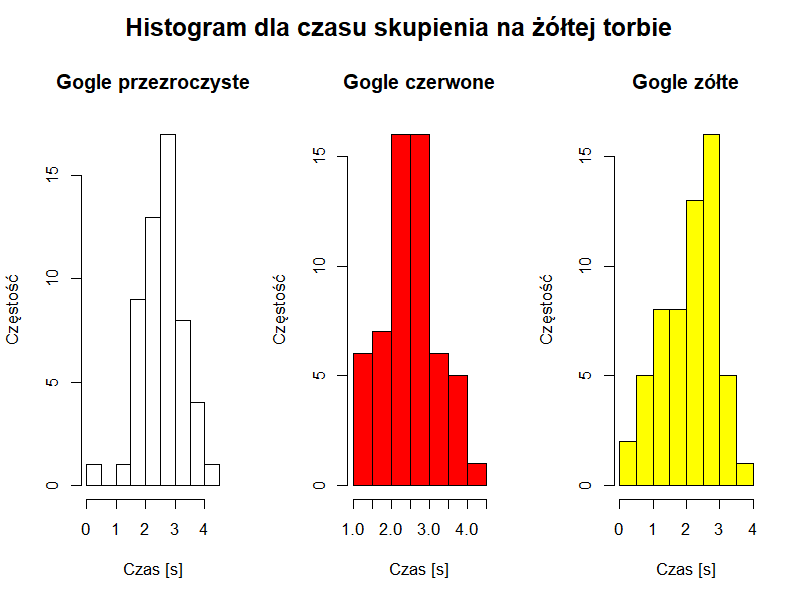
\includegraphics{./../res_plots/Histogram_dla_czasu_skupienia_na_żółtej_torbie.png}%
    %     }
    %     \label{fig:histTFD_yBag}
    % \end{figure}
    \begin{figure}[H]
        \centering
        \caption{Wykres pudełkowy dla zmiennej TFD dla obiektu żółta torba (yellow bag).}
        \resizebox{0.7 \columnwidth}{!}{%
        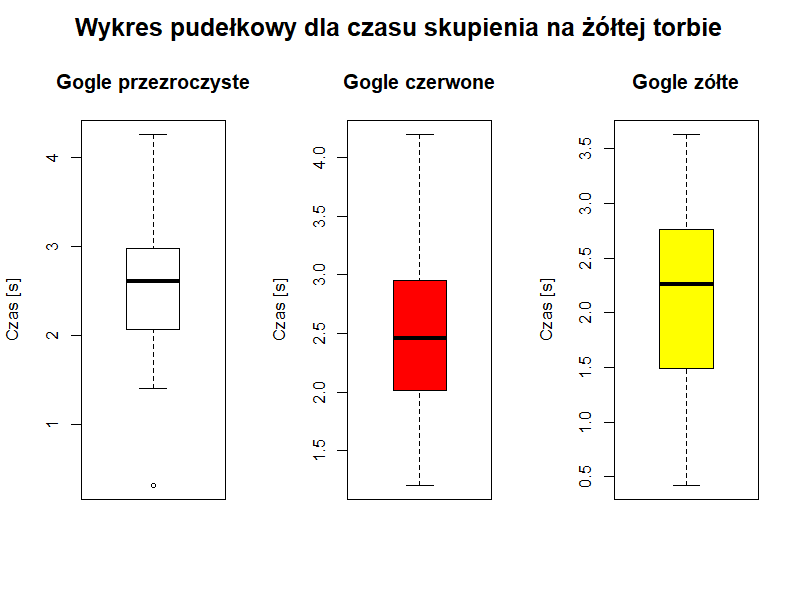
\includegraphics{./../res_plots/Wykres_pudełkowy_dla_czasu_skupienia_na_żółtej_torbie.png}%
        }
        \label{fig:boxTFD_yBag}
    \end{figure}

    \subsection{Równoliczność grup} %TODO
    
    \subsection{Normalność zmiennej w grupach}
    \begin{table}[H]
        \centering
        \caption{Wyniki testu Shapiro-Wilka dla czasu skupienia na żółtej torbie (bez przekształceń).}
        \begin{tabular}{|c|c|c|}%
            \hline
            \bfseries Kolor okularów & \bfseries Wartość p & \bfseries Czy rozkład normalny% specify table head
            \csvreader[head to column names]{./../res_tables/yBag_shapiro_default.csv}{}% use head of csv as column names
            {\\\hline\kolorGogli & \num{\shapiroP} & \czyNormalny}% specify your columns here
            \\\hline    
        \end{tabular}
        \label{tab:shapiroYBagDefault}
    \end{table}
    \begin{figure}[H]
        \centering
        \caption{Histogram dla czasu skupienia na żółtej torbie (bez przekształceń).}
        \resizebox{0.7 \columnwidth}{!}{%
        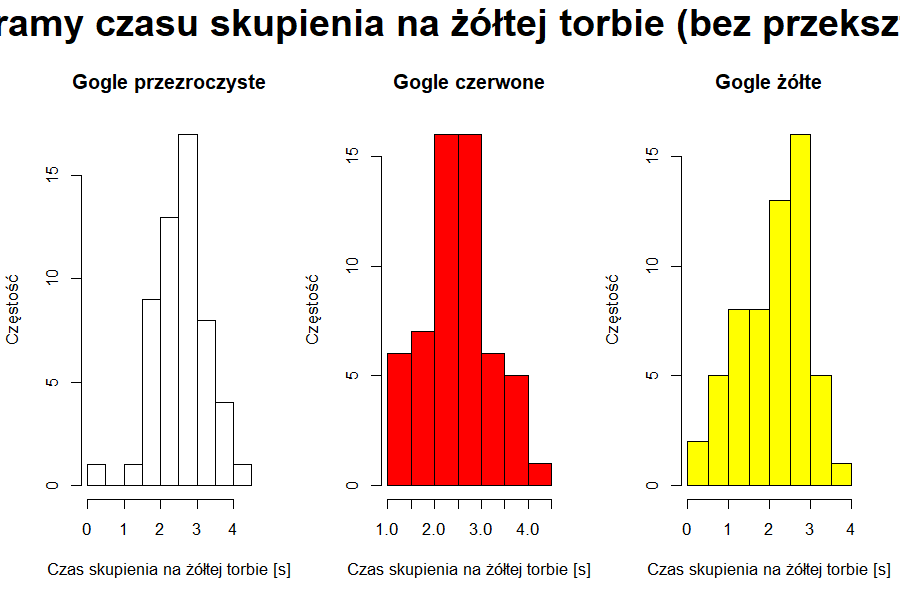
\includegraphics{./../res_plots/historgram_dla_TFD_yBag_default.png}%
        }
        \label{fig:histYBagDefault}
    \end{figure}

    \begin{table}[H]
        \centering
        \caption{Wyniki testu Shapiro-Wilka dla czasu skupienia na żółtej torbie (pierwiastek z X).}
        \begin{tabular}{|c|c|c|}%
            \hline
            \bfseries Kolor okularów & \bfseries Wartość p & \bfseries Czy rozkład normalny% specify table head
            \csvreader[head to column names]{./../res_tables/yBag_shapiro_x^0.5.csv}{}% use head of csv as column names
            {\\\hline\kolorGogli & \num{\shapiroP} & \czyNormalny}% specify your columns here
            \\\hline    
        \end{tabular}
        \label{tab:shapiroYBagPow0.5}
    \end{table}
    \begin{figure}[H]
        \centering
        \caption{Histogram dla czasu skupienia na żółtej torbie (pierwiastek z X).}
        \resizebox{0.7 \columnwidth}{!}{%
        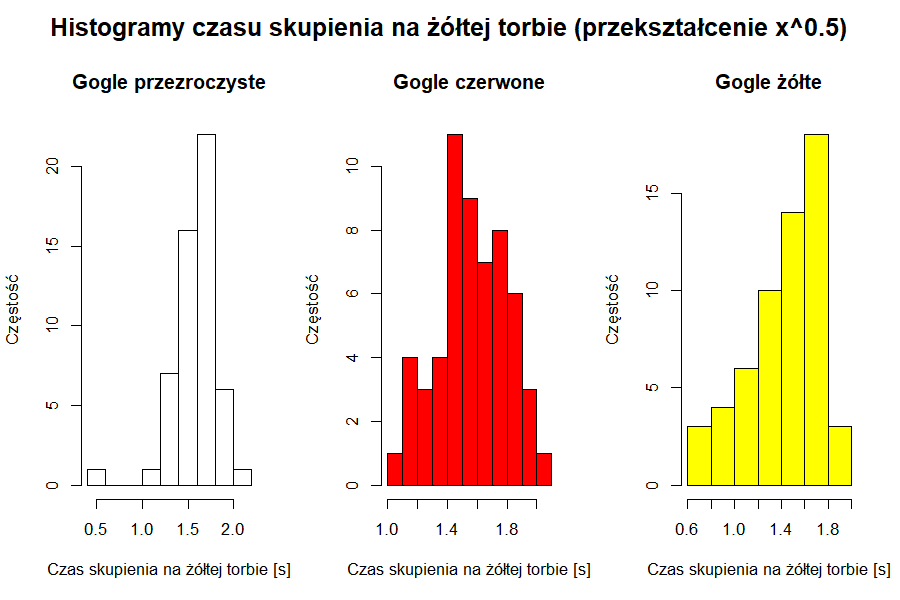
\includegraphics{./../res_plots/historgram_dla_TFD_yBag_x^0.5.png}%
        }
        \label{fig:histYBagPow0.5}
    \end{figure}

    \begin{table}[H]
        \centering
        \caption{Wyniki testu Shapiro-Wilka dla czasu skupienia na żółtej torbie (pierwiastek kwadratowy z X).}
        \begin{tabular}{|c|c|c|}%
            \hline
            \bfseries Kolor okularów & \bfseries Wartość p & \bfseries Czy rozkład normalny% specify table head
            \csvreader[head to column names]{./../res_tables/yBag_shapiro_x^0.25.csv}{}% use head of csv as column names
            {\\\hline\kolorGogli & \num{\shapiroP} & \czyNormalny}% specify your columns here
            \\\hline    
        \end{tabular}
        \label{tab:shapiroYBagPow0.25}
    \end{table}
    \begin{figure}[H]
        \centering
        \caption{Histogram dla czasu skupienia na żółtej torbie (pierwiastek kwadratowy z X).}
        \resizebox{0.7 \columnwidth}{!}{%
        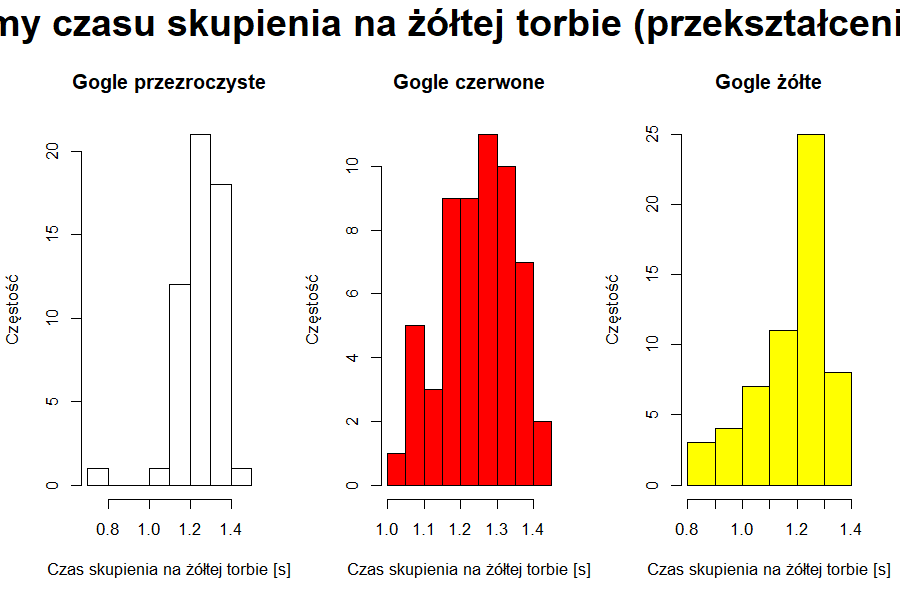
\includegraphics{./../res_plots/historgram_dla_TFD_yBag_x^0.25.png}%
        }
        \label{fig:histYBagPow0.25}
    \end{figure}

    \begin{table}[H]
        \centering
        \caption{Wyniki testu Shapiro-Wilka dla czasu skupienia na żółtej torbie (logarytm z X).}
        \begin{tabular}{|c|c|c|}%
            \hline
            \bfseries Kolor okularów & \bfseries Wartość p & \bfseries Czy rozkład normalny% specify table head
            \csvreader[head to column names]{./../res_tables/yBag_shapiro_log(x).csv}{}% use head of csv as column names
            {\\\hline\kolorGogli & \num{\shapiroP} & \czyNormalny}% specify your columns here
            \\\hline    
        \end{tabular}
        \label{tab:shapiroYBagLog}
    \end{table}
    \begin{figure}[H]
        \centering
        \caption{Histogram dla czasu skupienia na żółtej torbie (logarytm z X).}
        \resizebox{0.7 \columnwidth}{!}{%
        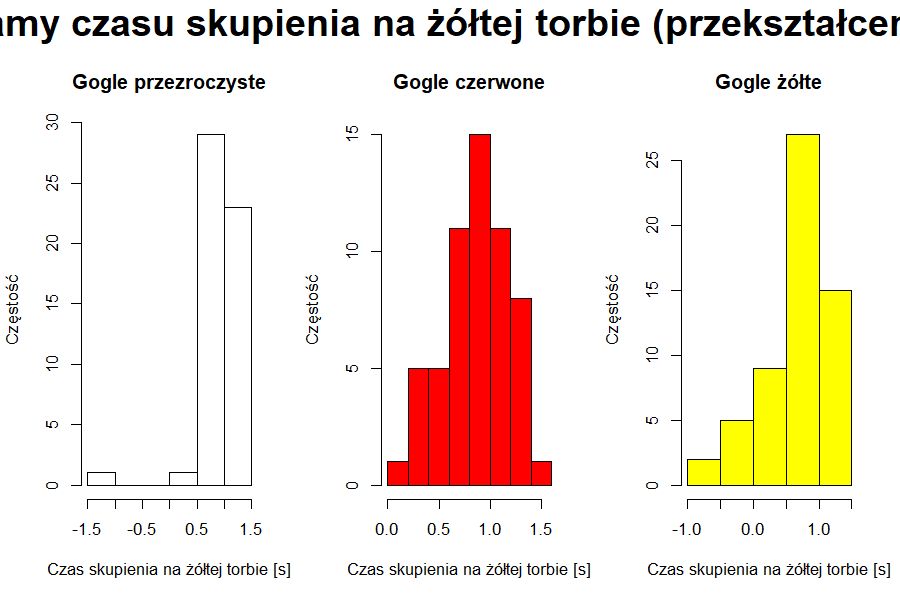
\includegraphics{./../res_plots/historgram_dla_TFD_yBag_log(x).png}%
        }
        \label{fig:histYBagLog}
    \end{figure}


    \subsection{Równość wariancji w grupach} %TODO
    \subsection{Równość średnich w grupach} %TODO
        \subsubsection{Uzasadnienie wyboru testu na podstawie wyników analiz z punktów 2-5} %TODO
        \subsubsection{Przeprowadzenie testu - wynik i wnioski} %TODO
    \subsection{Wpływ doświadczenia na zmienną TFD} %TODO
\section{Analiza wrażliwości} %TODO
\section{Wnioski i podsumowanie} %TODO

\end{document}